\documentclass[a4paper]{article}
\usepackage[english]{babel}
\usepackage[utf8]{inputenc}

% mathermatics
\usepackage{amssymb} % useful math symbols
\usepackage{amsmath} % more useful math
\usepackage{bm} % for bold matrices

% references and equation numbering
\usepackage{hyperref}
\usepackage{cleveref}
\usepackage{autonum}

% graphics
\usepackage{graphicx}
\usepackage{float}    % for more accurate graphics placement
\usepackage{fancyhdr} % for top header

% formatting
\usepackage{enumitem} % provides easy change of labels in enumerate environment
\usepackage[top=3cm, bottom=3cm, width=17cm]{geometry} % for smaller page margins

% colors
\usepackage{xcolor}

%% coding
% 
% see https://github.com/gpoore/minted for info
% uncomment this after you have completed the required installation
%
%\usepackage{minted} 
%\definecolor{codeBgColor}{RGB}{240,240,240}
%

\newcommand{\matr}[1]{\bm{#1}}


% very simple alias, \ex{} becomes the same as \subsubsection*{}
% TIP: remove the * in the line below if you want it numbered
\newcommand{\ex}[1]{\subsubsection*{#1}}




%Begining of the document
\begin{document}

\pagestyle{fancy} % use pagestyle with simple header (from fancyhdr)

%\pagenumbering{gobble} % uncomment to remove pagenumbering (in case of single page document)
\fancyhead[L]{TMA4140 Diskret Matematikk}
\fancyhead[C]{\textbf{Øving 9}}
\fancyhead[R]{Otto Lote 748704}


\subsection*{Section 9.6}
\ex{Exercise 9}

The directed graph is not a partial order as it is not transitive since there
is an edge \(a \to b\) and \(b \to c\) but no edge \(b \to c\).


\ex{Exercise 18}

\begin{enumerate}[label=\alph*), start=2] 
    \item open, opened, opener, opera, operand
\end{enumerate}


\ex{Exercise 27} 

(a, a),(a, g),(a, d),(a, e),(a, f), \\
(b, b),(b, g),(b, d),(b, e),(b, f), \\
(c, c),(c, g),(c, d),(c, e),(c, f), \\
(d, d), \\
(e, e), \\
(f, f), \\
(g, d),(g, e),(g, f),(g, g)

\ex{Exercise 32}

\begin{enumerate}[label=-]
    \item Elements \(l\) and \(m\) are maximal elements
    \item Elements \(a\), \(b\) and \(c\) are minimal elements
    \item There is no greatest element
    \item There is no least element
    \item \(k\), \(l\) and \(m\) are upper bounds of \(\{a, b, c\}\)
    \item The least upper bound of \(\{a, b, c\}\) is \(k\)
    \item There is no lower bound for \(\{f, g, h\}\)
    \item Because of g) there is no greatest lower bound
\end{enumerate}

\subsection*{Section 10.2}
\ex{Exercise 18}

For a graph with \(n\) where \(n \leq 2\) vertices the degree of one of those
    vertices can be at most of degree \(n - 1\) and at least of degree 1, this
    means we have \(n-1\) different possible degrees. For \(n\) vertices and a
    maximum of \(n-1\) unique degrees, at least two of them must have the same
    degree.

\ex{Exercise 22}

The graph is bipartite where \(a, c\) is on one side, and \(b, d, e\) on the other. 

\ex{Exercise 26}

\begin{enumerate}[label=\alph*)]
    \item \(K_n\) is bipartite only for \(n=2\)
    \item \(C_n\) is bipartite for \(n \leq 4\) and \(n\) is even.
    \item \(W_n\) is not bipartite for any \(n\).
\end{enumerate}

\ex{Exercise 55}

A regular graph of degree 4 with \(n\) vertices has \(\frac{4n}{2}\) edges,
    which means the number of nodes is half the number of edges, which is 5
    nodes in this case. 

\subsection*{Section 10.3}

\ex{Exercise 17}

\begin{figure}[H]
    \centering
    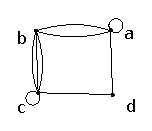
\includegraphics[width=0.3\textwidth]{10-3-17.eps}
\end{figure}

\ex{Exercise 19}

\[
    \begin{bmatrix}
        0 & 1 & 0 & 0 \\
        0 & 1 & 1 & 0 \\
        0 & 1 & 1 & 1 \\
        1 & 0 & 0 & 0 \\
    \end{bmatrix}
\]


\ex{Exercise 23}

\begin{figure}[H]
    \centering
    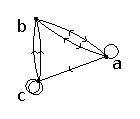
\includegraphics[width=0.3\textwidth]{10-3-23.eps}
\end{figure}

%% uncomment this if you need references. Edit the .bbl file with your references
%% and use "\cite{bibitem-label}" to cite
%\bibliography{template}

\end{document}

